\section{Auswertung}
\label{sec:Analysis}
Diese Auswertung ist unterteilt in eine Spektrometer-Messung in \autoref{sec:spec}, eine Messung über die radiale Symmetrie in \autoref{sec:radial}, die Simulationsergebnisse in \autoref{sec:sim} und die Intensitätsmessung zur Bestimmung der Dämpfungslänge in \autoref{sec:intensity}.
\subsection{Spektrometer-Messung}
\label{sec:spec}
Als erstes wird die Spektrometer-Messung durchgeführt. Das gemessene Signal ist in der \autoref{fig:spectra} eingezeichnet. Die Messung wurde einmal mit Raumlicht gemessen und einmal ohne Raumlicht.\\\\
\begin{figure}
    \centering
    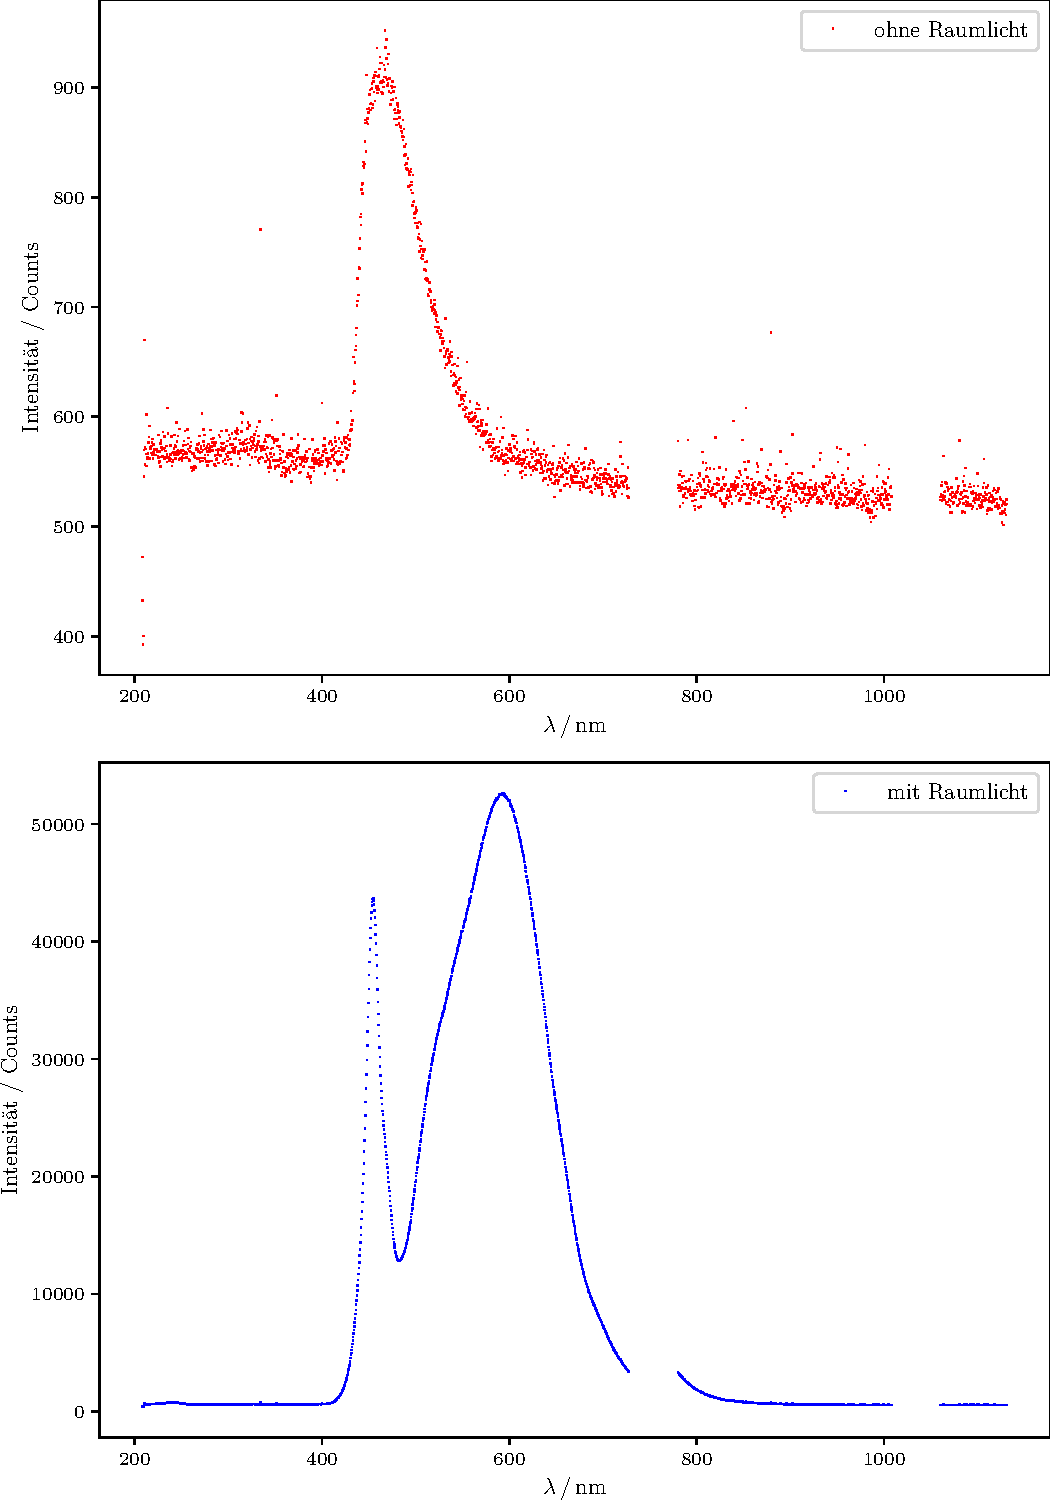
\includegraphics[width=10cm, keepaspectratio]{build/spectra.pdf}
    \caption{Messungen des Spektrometers mit Raumlicht an und aus.}
    \label{fig:spectra} 
 \end{figure}
 Bei der Messung ohne Raumlicht zeigt sich ein klarer Peak bei etwa $\SI{460}{\nano\meter}$ auf der Höhe des Hintergrundrauschens, das hier bei etwa 570 Counts liegt. Bei angeschaltetem Raumlicht zeigt sich ein vielseitigeres Profil mit einem Peak bei einer ähnlichen Wellenlänge von ungefähr $\SI{454}{\nano\meter}$ und einer breiteren Kurve. Bei dem Peak vor dem größeren Lichtspektrum handelt es sich vermutlich nicht direkt um die Diode, auch wenn diese dem Farbspektrum ähnelt, da die gemessene Intensität bei dem angeschalteten Raumlicht bei etwa $\num{43677.8}$ Counts liegt und damit viel größer ist als die Intensität von der Photodiode ohne Raumlicht mit etwa $\num{936.4}$ Counts.\\\\
 Als Nächstes werden die "Dark Counts" (DC) von dem gemessenen Signal abgezogen. Das Resultat wird in \autoref{fig:spectra_dc} dargestellt.\\\\
 \begin{figure}
    \centering
    
\includegraphics[width=10cm, keepaspectratio]{build/spectra_dc.pdf}
    \caption{Korrigierte Intensitäten der Messung von \autoref{fig:spectra}, indem die "Dark Counts" (DC) vom Signal abgezogen wurden.}
    \label{fig:spectra_dc}
 \end{figure}
 Ähnlich wie bei der \autoref{fig:spectra} ist der Peak der Photodiode ohne Raumlicht und abgezogenen Dark Counts klar erkennbar. Ist jedoch das Raumlicht eingeschaltet, dann ist eine Verzerrung des Peaks trotz abgezogenen Dark Counts sichtbar, weshalb die folgenden Messungen ohne Raumlicht fortgeführt werden.
 \subsection{Radiale Messung}
 \label{sec:radial}
 Für die radiale Messung wurde der horizontale Winkel $h$ von $\SI{-18}{\degree}$ bis $\SI{34.5}{\degree}$ und der vertikale Winkel $v$ von $\SI{-6}{\degree}$ bis $\SI{34.5}{\degree}$ jeweils eingestellt und mithilfe des Spektrometers für die verschiedenen Wellenlängen $\lambda$ eine jeweilige Intensität ermittelt. Danach wurden alle Intensitäten der verschiedenen Wellenlängen summiert, um eine gesamte Intensität zu bestimmen. Das Resultat ist in der \autoref{fig:radial} in ein zwei-dimensionales Histogramm dargestellt.\\\\
 \begin{figure}
    \centering
    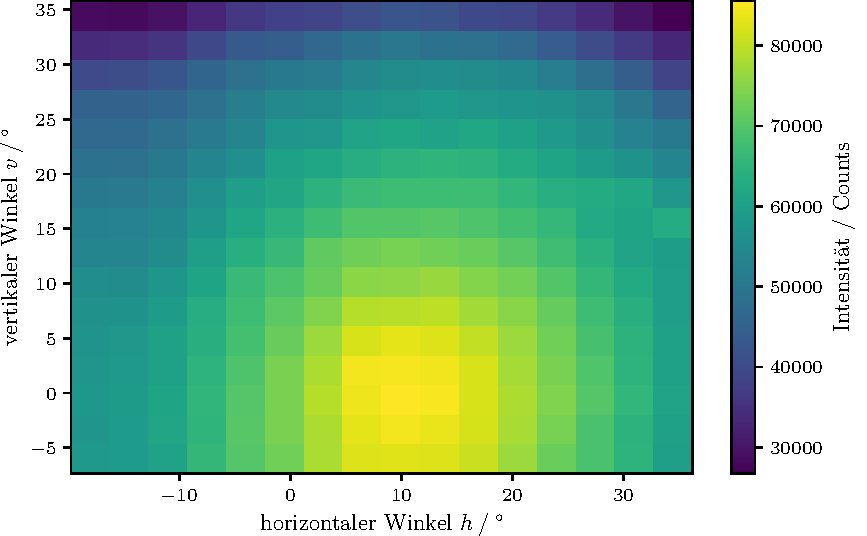
\includegraphics[width=10cm, keepaspectratio]{build/radial.pdf}
    \caption{Ein zwei-dimensionales Histogramm der gemessenen Intensitäten in Abhängigkeit des horizontalen Winkels $h$ und des vertikalen Winkels $v$.}
    \label{fig:radial}
 \end{figure}
 Es zeigt sich eine klare radiale Symmetrie, die durch die Faser bestimmt wird. Desweiteren nimmt die Intensität mit dem Zentrum nach Außen hin wie erwartet ab.
 \subsection{Simulation}
 \label{sec:sim}
 Die Simulation erstellt einen Datensatz der zunächst auf unphysikalische Photonen gefilert werden muss. Dafür wird zunächst der Radius der Faser bestimmt. Der Durchmesser ist in der Versuchsanleitung \cite{Anleitung} gegeben daraus schließt sich der Faserradius von $r_{\text{Faser}} = \SI{0.125}{\milli\meter}$. Dann wird aus den Simulationswerten $y_{\text{exit}}$ und $z_{\text{exit}}$ ein radialer Ausgangspunkt aus der Faser $r_{\text{exit}}$ mithilfe von $r_{\text{exit}} = \sqrt{y_{\text{exit}}^2 + z_{\text{exit}}^2} \leq r_{\text{Faser}}$ bestimmt. Dieser Wert lässt als Bedingung nur noch die Photonen in dem Ergebnis, welche auch nur innerhalb der Faser hätten austreten können. Ebenso werden die Photonen gefiltert die mit der Rayleigh Streuung heraus gestreut werden.\\
 Danach wird ein neuer Raumwinkel $\Theta$ eingeführt. Dieser beschreibt den Winkel von den simulierten Photonen zu der Faserachse und leitet sich aus der Formel $p_x = |\vec{p}| \cdot \cos{\Theta}$ her. Dabei ist $p_x$ bekannt in der Simulation und $\vec{p}$ ist normiert und damit gegeben als $|\vec{p}| = 1$. Es folgt die Formel
 \begin{equation}
    \Theta = \arccos{p_x}.
    \label{eqn:theta}
 \end{equation}
Um die Photonen in den Bereichen ''Cladding'' und ''Core'' zu unterteilen, werden diese mithilfe der Einträge von ''length\_clad'' sortiert. Dieser Wert stellt die zurückgelegte Länge im Mantel dar und identifiziert die ''Core''-Photonen direkt, da diese nicht in den Mantel eindringen. Die jeweiligen kritischen Winkel zeigen dabei den Grenzwert der inneren Totalreflexion in der korrespondierenden Schicht an. Dafür werden die Brechnungsindizes von dem Kern $n_{\text{core}}$, der ersten Ummantelung $n_{\text{clad1}}$ und von der zweiten Ummantelung $n_{\text{clad2}}$ benötigt. Diese werden erneut aus dem Skript entnommen \cite{Anleitung} und sind damit gegeben als $n_{\text{core}} = \num{1.6}$, $n_{\text{clad1}} = \num{1.49}$ und $n_{\text{clad2}} = \num{1.42}$. Die kritischen Winkel lassen sich bestimmen mit
 \begin{equation}
    \Theta_{\text{krit, core}} = \arcsin{\left(\frac{n_{\text{clad1}}}{n_{\text{core}}}\right)} \approx \SI{21.3695}{\degree} \quad \text{und} \quad \Theta_{\text{krit, clad}} = \arcsin{\left(\frac{n_{\text{clad2}}}{n_{\text{core}}}\right)} \approx \SI{27.4392}{\degree}.
    \label{eqn:theta_krit}
 \end{equation}
Die Ergebnisse zu der simulierten Intensität in Abhängigkeit von $\Theta$ und unterteilt in ''Cladding'' und ''Core'' befinden sich in der \autoref{fig:SimData}. Ebenfalls sind die kritischen Winkel von dem Übergang ''Core'' zu ''Cladding 1'' und dem Übergang ''Cladding 1'' zu ''Cladding 2'' eingezeichnet.
 \begin{figure}
    \centering
    
\includegraphics[width=10cm, keepaspectratio]{build/SimData.pdf}
    \caption{Die simulierten Intensitäten in ein Histogramm gegen den Winkel $\Theta$ aufgetragen.}
    \label{fig:SimData}
\end{figure}
Es ist ein linearer Anstieg der ''Core''-Photonen erkennbar. Dies lässt sich daraus herleiten, dass der Raumwinkel definiert ist als $\text{d}\Omega = \sin{\Theta}\, \text{d}\Theta \text{d}\Phi$ und für kleine Winkel ist $\sin{\Theta} \approx \Theta$ und damit linear für den Anfang. Der kritische Winkel von den ''Core''-Photonen liegt auf dem Maximum der Intensität, da ab diesem Punkt die Photonen in den Mantel übergehen. Es werden jedoch noch weitere Photonen über dem kritischen Winkel hinaus gemessen, da die Berechnung des kritischen Winkels eine meridionale Laufbahn voraussetzt. Diese ist jedoch nur für die Photonen bestimmt, die sich genau auf der Faserachse befinden. Die Photonen für die diese Voraussetzung nicht gilt, breiten sich durch wiederholten Totalreflexionen an den Grenzflächen entlang der Faser aus. Da dies den tatsächlichen Winkel der Photonen zur Grenzfläche verändert, sind auch noch ''Core''-Photonen bei einem größeren Winkel als den kritischen Winkel erlaubt. Da dies jedoch nur noch wenige Laufbahnen zulässt, ist die Intensität darüber hinaus stark unterdrückt, wie auch in der \autoref{fig:SimData} zu sehen ist.\\
Diese Begründung wird von den Daten der ''Cladding''-Photonen unterstützt, da die simulierten Werte alle oberhalb des kritischen Winkels $\Theta_{\text{krit, core}}$ sind und damit keine Totalreflexion innerhalb des Mantels ermöglichen würden, sodass diese in den Mantel übergehen. Die ''Cladding''-Photonen werden ebenfalls wie auch bei den ''Core''-Photonen ab dem kritischen Winkel $\Theta_{\text{krit, clad}}$ stark unterdrückt. Der Grund wieso die Photonen bei etwa $\SI{45}{\degree}$ nicht mehr ''gemessen'' werden, ist vermutlich, dass die Photonen zu stark unterdrückt werden unter der Bedingung der Totalreflexion bis hin zum kritische Winkel von der äußeren Umantelung zur Luftoberfläche. Dieser wird  mit $n_{\text{Luft}} \approx 1$ ungefähr bei $\Theta_{\text{krit, clad2}} = \arcsin{\left(\frac{n_{\text{Luft}}}{n_{\text{core}}}\right)} \approx \SI{51.3}{\degree}$ liegen.\\\\
Als nächstes wird der minimale Abstand zur Faserachse der einzelnen Photonen bestimmt. Da die Photonbahn eines Photons, das nicht auf der Faserachse bewegt, eine Gerade ist mit mehreren Reflexionen wird der minimale Abstand durch die Formel für den minimalen Abstand zweier Geraden im Raum bestimmt. Dabei ist die zweite Geraden auf der $x$-Achse. Dadurch folgt die Formel
\begin{equation*}
    r_{\text{min}} = \frac{|\vec{r}_0 \cdot \left(\vec{p} \times \vec{e}_x\right)|}{\left(\vec{p} \times \vec{e}_x\right)}.
    \label{eqn:r_min_alt}
\end{equation*}
Aus den Kreuzprodukten ergibt sich die Formel
\begin{equation}
    r_{\text{min}} = \frac{|y_0 p_z - z_0 p_y|}{\sqrt{p_y^2+p_z^2}}.
    \label{eqn:r_min}
\end{equation}
Die \autoref{eqn:r_min} gilt nur für Impulsvektoren die nicht parrallel der $x$-Achse laufen. Für $\vec{p} \parallel \vec{e}_x$ gilt:
\begin{equation}
    r_{\text{min, }\parallel} = \sqrt{y_0^2+z_0^2}.
    \label{eqn:r_min_parallel}
\end{equation}
Die Ergebnisse werden in der \autoref{fig:hist2d} für die ''Core''- und die ''Cladding''-Photonen in Abhängigkeit des Winkels $\Theta$ und des minimalen Abstandes zur Faserachse $r_\text{min}$ zusammengetragen.
\begin{figure}
    \centering
    
\includegraphics[width=10cm, keepaspectratio]{build/hist2d_core_clad.pdf}
    \caption{Ein zwei-dimensionales Histogramm von den simulierten Intensitäten in Abhängigkeit von dem minimalen Abstand zur Faserachse $r_{\text{min}}$ und dem Winkel $\Theta$.}
    \label{fig:hist2d}
\end{figure}
Unter der Betrachtung der Formel aus dem Skript \cite{Anleitung}
\begin{equation}
    \Theta_{\text{refl}} = \arcsin{\left(\sqrt{1-\frac{r_{\text{min}}^2}{r_{\text{core}}^2}}\sin{\Theta}\right)}
    \label{eqn:skript}
\end{equation}
ergibt sich, dass für kleine $r_{\text{min}}$, also für Photonen nahe der Faserachse, $\Theta_{\text{refl}} \approx \Theta$ ist und für große  $r_{\text{min}}$, also Photonen weiter außerhalb, der Reflexionswinkel $\Theta_{\text{refl}}$ kleiner ist als der Winkel zur Faserachse $\Theta$. Dies impliziert, dass nur große $\Theta$-Werte möglich sind mit größeren minimalen Abstand zur Faserachse $r_{\text{min}}$. Genau das lässt sich auch in der \autoref{fig:hist2d} wiedererkennen. Darüber hinaus sind die Grenzlinien, definiert durch die \autoref{eqn:skript} bei $\Theta_{\text{refl}} = \Theta_{\text{krit, core}}$ mit dem Abstand von der Faserachse zu der Grenzfläche von dem Kern $r_{\text{core}}= \SI{0.11}{\milli\meter}$ \cite{Anleitung} und $\Theta_{\text{refl}} = \Theta_{\text{krit, clad}}$ mit dem Abstand von der Faserachse zu der Grenzfläche von der ersten Ummantelung $r_{\text{clad1}}= \SI{0.1175}{\milli\meter}$ \cite{Anleitung}, mit eingezeichnet. Diese Grenzlinie stellt auch die simulierte Grenzlinie dar, ab welchen Winkeln $\Theta$ keine Photonen mehr ''gemessen'' werden.\\\\
Der letzte Schritt der Auswertung der Simulation ist die Bestimmung der Dämpfungslänge $\Lambda$ für verschiedene Winkel. Dabei wird erneut der Winkel $\Theta$, also der Winkel des Photons zur Faserachse verwendet.\\
Dieser unterscheidet sich insofern von der Messung aus dem \autoref{sec:intensity}, dass $\Theta$ Aussagen darüber trifft, wie das Photon an dem Punkt der Erzeugung zu der Faserachse verläuft und die eigentlichen Winkel der Messung aus der Intensitätsmessung sind jedoch Angaben über den Austrittswinkel am Faserende.
Danach werden die Photonen gezählt, die in einem festen Winkelbereich $\Theta$ von $\SI{0}{\degree}\pm\SI{2}{\degree}$ bis $\SI{36}{\degree}\pm\SI{2}{\degree}$ liegen. Dies wird dann in Abhängigkeit der Anregungsposition ''gpsPosX'' von $\SI{100}{\milli\meter}$ bis $\SI{2400}{\milli\meter}$ in der \autoref{fig:atten} dargestellt. Desweiteren wird ein Fit der Form
\begin{equation*}
    I_{\text{fit}}\left(x\right) = I_0 \cdot \exp^{-\frac{x}{\Lambda_{\text{eff}}\left(\Theta , x\right)}} \quad \text{mit} \quad x = \text{''gpsPosX''}
    \label{eqn:atten_fit}
\end{equation*}
durch die simulierten Messwerte für die verschiedenen Winkel $\Theta$ gezeichnet.
\begin{figure}
    \centering
    
\includegraphics[width=10cm, keepaspectratio]{build/atten.pdf}
    \caption{Die simulierte Intensität für die Winkel $\Theta$ von $\SI{0}{\degree}\pm\SI{2}{\degree}$ bis $\SI{36}{\degree}\pm\SI{2}{\degree}$ und verschiedenen "gpsPosX"-Werten von $\SI{100}{\milli\meter}$ bis $\SI{2400}{\milli\meter}$.}
    \label{fig:atten}
\end{figure}
Die Intensität fällt wie erwartet exponentiell mit der Anregungsposition $x$ ab. Es zeigt sich, dass die Dämpfungslänge für verschiedene Winkel $\Theta$ stark schwanken. Das liegt daran, dass es sich dabei um eine effektive Größe handelt und Verluste von ''Core''- und ''Cladding''-Photonen unter der Variable $\Lambda_{\text{eff}}\left(\Theta , x\right)$ versucht zu beschreiben. Diese Verluste beziehen sich auf die Abschwächungen im Material durch Absorption oder Streuung als auch auf die Reflexionsverluste an den Grenzflächen. Die Ergebnisse sind in der \autoref{tab:atten} dokumentiert.
\begin{table}
    \centering
    \caption{Die effektive Dämpfungslängen für verschiedene Winkel $\Theta$.}
    \label{tab:atten}
    \begin{tabular}{c c}
    \toprule
    {$\Theta \pm \SI{2}{\degree} \mathbin{/} \si{\degree}$} & {$\Lambda_{\text{eff}} \mathbin{/} \si{\milli\meter}$} \\
    \midrule
     0 & 4967 \\
     4 & 5142 \\
     8 & 5255 \\
    12 & 5222 \\
    16 & 5145 \\
    20 & 5100 \\
    24 & 5328 \\
    28 & 5068 \\
    32 & 4919 \\
    36 & 4868 \\
    \bottomrule
  \end{tabular}
\end{table}
Dadurch dass die Intensitäten exponentiell abfallen, folgt daraus, dass wenn ein Photon eine längere Weglänge durch die Faser läuft bzw. häufiger reflektiert wird, die effektive Reichweite damit verkürzt wird.
Die effektiven Dämpfungslängen $\Lambda_{\text{eff}}$ liegen dabei in dem Bereich von $\SI{4868}{\milli\meter}$ bis zu $\SI{5328}{\milli\meter}$.
\subsection{Intensitätsmessung}
\label{sec:intensity}
Für die Intensitätsmessung wird der Winkel $h = \SI{10}{\degree}$ eingestellt, wo sich das Intensitätsmaximum befindet und $v$ von $\SI{0}{\degree}$ bis $\SI{36}{\degree}$ eingestellt und die Intensität für die verschiedenen $x$-Werten von $\SI{0}{\milli\meter}$ bis $\SI{2400}{\milli\meter}$ gemessen. Es folgen die Resultate in der \autoref{fig:intensity}. Genauso wie in \autoref{sec:sim} wird ein Fit der Form aus der \autoref{eqn:atten_fit} durch die Messwerte der verschiedenen Winkel $v$ erstellt.
\begin{figure}
    \centering
    
\includegraphics[width=10cm, keepaspectratio]{build/intensity.pdf}
    \caption{Die gemessenen Intensitäten für einen festen horizontalen Winkel $h = \SI{10}{\degree}$ am Intensitätsmaximum und verschiedenen vertikalen Winkeln $v$ von $\SI{0}{\degree}$ bis $\SI{36}{\degree}$ und verschiedenen $x$-Werten von $\SI{0}{\milli\meter}$ bis $\SI{2400}{\milli\meter}$.}
    \label{fig:intensity}
\end{figure}
Die Ergebnisse liefern verschiedene Dämpfungslängen absteigend von $\SI{1530}{\milli\meter}$ bis zu $\SI{2182}{\milli\meter}$ und sind in der \autoref{tab:intensity} dargestellt.
\begin{table}
    \centering
    \caption{Die Dämpfungslängen für verschiedene Winkel $v$ mit einem konstanten Winkel $h$.}
    \label{tab:intensity}
    \begin{tabular}{c c}
    \toprule
    {$v \mathbin{/} \si{\degree}$} & {$\Lambda \mathbin{/} \si{\milli\meter}$} \\
    \midrule
     0 & 2182 \\
     4 & 2048 \\
     8 & 1957 \\
    12 & 1952 \\
    16 & 1898 \\
    20 & 1782 \\
    24 & 1735 \\
    28 & 1674 \\
    32 & 1587 \\
    36 & 1530 \\
    \bottomrule
  \end{tabular}
\end{table}
Ebenso sind zwei Kanten in den Verläufen sichtbar. Das könnte daran liegen, dass bei der $x$-Position die Faser leicht beschädigt ist, welche die Dämpfungslängen der jeweiligen Fit-Kurven verfälschen. Ebenso ist eine mögliche ungewollte externe Reflexion oder Lichtquelle möglich. Für den Fall, dass man erst die Messwerte ab dem letzten Knick verwendet, entstehen dadurch die Dämpfungslängen absteigend von $\SI{2261}{\milli\meter}$ bis zu $\SI{3715}{\milli\meter}$. Diese Berechnung wird jedoch ansonsten nicht weiter berücksichtigt in dieser Auswertung und dient nur als Referenz der Sensibilität des Zustandes der Faser oder den äußeren Einwirkungen. Grundsätzlich liegt der Bereich der Dämpfungslängen in dem erwarteten Spektrum von mehreren tausend Millimetern.